\section{PROBLEM DEFINITION}
\label{sec:proposed_approach}

The objective of the superpixel propagation is
therefore to find the best labeling $L$ for every superpixel $p$
(with $L_p \in {0,1,...N-1}$) between a pair
of frames ($I_{1}$,$I_{2}$), but holding a flow-like behavior.
   \begin{figure}[thpb]
      \centering
      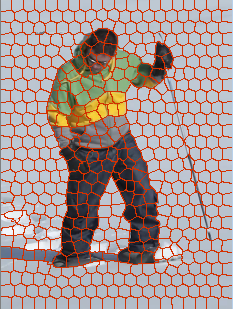
\includegraphics[height=0.22\textheight]{images/segmentation.png}
      \caption{SLIC super segmentation in the Snow Shoes sequence.}
      \label{figurelabel_segmentation}
   \end{figure}
Thus, the superpixelization should maintain certain
regularity in size within a single frame. Some super
pixel techniques can cope with this requirement \cite{c9}\cite{c10}.
For the experiments presented in this work, we prefer
the SLIC (Fig. \ref{figurelabel_segmentation}) method \cite{c9}, which usually gives
good results in homogeneity of the superpixelization.
The proposed steps to solve the propagation problem
assume this requirement is hold. For other kind of the
techniques, other approaches should be followed.

%\addtolength{\textheight}{-3cm}   % This command serves to balance the column lengths
                                  % on the last page of the document manually. It shortens
                                  % the textheight of the last page by a suitable amount.
                                  % This command does not take effect until the next page
                                  % so it should come on the page before the last. Make
                                  % sure that you do not shorten the textheight too much.

%%%%%%%%%%%%%%%%%%%%%%%%%%%%%%%%%%%%%%%%%%%%%%%%%%%%%%%%%%%%%%%%%%%%%%%%%%%%%%%%
\subsection{Energy Formulation}

Inspired by a large number of optical flow and stereo
techniques \cite{c7}\cite{c12}\cite{c13}, the super-pixel propagation can be
modeled with pairwise Markov Random Fields. If
the matching is performed with MAP inference, its
posterior probability is: 
\begin{equation}
 P(L|I_0,I_1) = \displaystyle \prod_{p \in \Omega} \mathrm{e}^{-D_p(L_p;I_0,I_1)} 
\prod_{p,q \in \mathcal{N}_p} \mathrm{e}^{-S_{p,q}(L_p;L_q)} 
\label{eq_prob}
\end{equation}

With $L$ the set of labels of the super pixels in $I_0$,
that match with those in $I_1$.
$ \mathcal{N}_p $ is a neighborhood of the
superpixel $p$, which defines its adjacency. Given this posterior probability,
the equivalent energy function can be directly obtained
by extracting the negative logarithm of the posterior,

\begin{equation}
E(L) = \displaystyle \sum_{p \in \Omega} -D_p(L_p;I_0,I_1) +
\sum_{p,q \in \mathcal{N}_p} -S_{p,q}(L_p,L_q)
\label{eq_energy}
\end{equation}

The terms $D$, and $S$ in \ref{eq_energy} stand for data and spatial as they
are popularly known in the MRF literature. The first
one determines how accurate is the labeling in terms
of consistency of the measured data (Color, Shape,
etc.). In the usual optical flow counterpart of this equation,
the data term corresponds to the pixel
brightness \cite{c7}\cite{c5}. However, as superpixels are a set
of similar (or somehow homogenous) pixels, an
adequate color based feature can be a low binned
histogram or its average color. So it can be written 
more precisely as

\begin{equation}
D_p(L_p;I_0,I_1) = \rho(h(p),h(p'))
\label{eq_Dp}
\end{equation}

Where $h(p)$ and $h(p')$ are the histograms of the super-
pixel $p$ and its correspondent superpixel in the
second frame ($I_1$). $rho$ can be replaced by the Bhattacharyya
 distance. Note that the low binned histogram or
average color gives certain robustness against noise,
and slowly changing colors between frames.
The spatial term is a penalty function for horizontal
and vertical changes of the vectors that have origin in
the centroid of the super-pixel of the first frame and
end in the centroid of the super-pixel of the second
frame.

\begin{equation}
S_{p,q}(L_p,L_q) = \lambda(p)
  \sqrt{\frac{|u_{p_c}-u_{q_c}|}{\|p_c-q_c\|}+ \frac{|v_{p_c}-v_{q_c}|}{\|p_c-q_c\|}}
\label{eq_Spq}
\end{equation}
\begin{center}
 where, $ \lambda(p) = (\rho(h(p),h(p')))^2 $ \\
\end{center}

In \ref{eq_Spq} the operator $\rho$ has the same meaning as in the
data term \ref{eq_Dp}. The histograms distance is nonetheless
computed between super pixels $p$ and $q$, which belong to
the same neighborhood. The super pixels
centroids are noted as $q_c$ and $p_c$, and $u$ and $v$ are the
horizontal and vertical changes between centroids.
This term is usual in the MRF formulation and has a
smoothing effect in superpixels that belong to the
same object. It has to be observed that when two
superpixels are different, thus, more probable to be
in different semantic groups within the image, the
term $\lambda$ allows them to have
matches that do not hold the smoothness prior with the same strength. 
It has to be noted that the proposed energy function is
highly non-convex and robust.

\subsection{Energy Minimization}

A fair amount of work had been dedicated to
discrete optimization techniques in computer vision,
leading to a couple of well-defined and widely tested
approaches to solve the pairwise MRF of labels \cite{c3}\cite{c4}.
However, some of the approaches restrict the
construction of the spatial term, and/or enforce
limitations in the number of labels \cite{c3}.
Because of the high amount of possible labels for 
each element in the proposed approach, the use of the
Fusion Moves \cite{c7} technique seems to be well suited.
This algorithm employs the Quadratic Pseudo-
Boolean Optimization (QPBO) graph-cut, to combine
incremental sets of proposal labeling, resulting a semi-
globally-optimal solution \cite{c4}.
Thus, the minimization starts by proposing a set of
possible solutions, and iteratively merge them with
the QPBO graph-cut technique. \\
The possible solutions that can be given depend on the kind of
problem that is intended to be solved. For example, in
stereo super-pixel matching, some assumptions
related to the cameras organization can be made to
generate solutions.
In a more generic sense, other assumptions can be
made towards option generation. For instance, for a
given super-pixel in the initial frame, in the second
frame the corresponding matching would be the most
similar one in terms of color, or the most similar un
terms of shape, or the spatially closer super-pixel.
More proposal solutions can be added by defining a
neighborhood in the second frame and select random
pairs from every neighborhood of every super-pixel
in the first frame. This is more suitable for problems
where the images are extracted from the same video
sequence. It is interesting to notice that different
assumptions for this neighborhood can lead to a
technique for generic image based retrieval, where
the total cost of matching can be used as metric.

\section{EXPERIMENTAL RESULTS}
The Fig. \ref{figurelabel_matches} shows some examples of superpixel
matching with the presented method. It can be seen
that the matching performs well even in difficult
cases, like the hands in the top row. It has to be noted
as well that even in superpixels where there is a lack
of texture, there is correct matching. This seems to be
the effect of enforcing the regularization between
superpixels that are close, but are also similar to
each other.

   \begin{figure}[thpb]
      \centering
      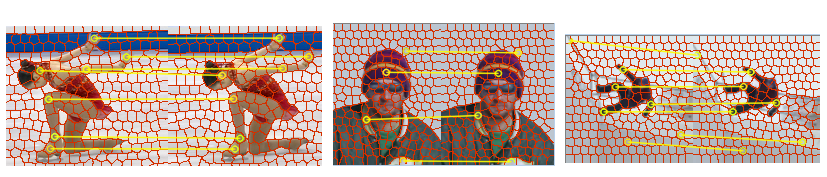
\includegraphics[height=0.33\textheight]{images/matches.png}
      \caption{The yellow lines show selected super-pixel
		matching between pairs of subsequent frames in a video
		with the proposed method. The video frames go from right
		to left.}
      \label{figurelabel_matches}
   \end{figure}
 
 Moreover, unlike most of the optical flow methods, superpixel flow extends 
 naturally for more distant frames. The Fig. \ref{figurelabel_matchessnow} shows
 results for larger separations between frames, without tweaking or adjusting any
 parameters. For this case, however, the matches in the textureless part of the scene
 are mostly invalids. Though this is expected because because of the aperture problem and
 heavy occlusions.
 
   \begin{figure}[thpb]
      \centering
      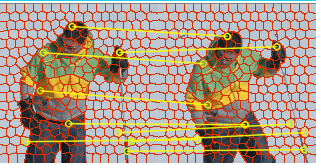
\includegraphics[height=0.1\textheight]{images/matches_snowshoes.png}
      \caption{The yellow lines show selected superpixel
		matching between a pair of distant frames in the Snow Shoes sequence.}
      \label{figurelabel_matchessnow}
   \end{figure}
   
\subsection{Superpixel propagation for object segmentation in videos}
The GrabCut algorithm proposed in \cite{c14}, offers a good deal in terms of
background-foreground separation from user interaction. A technique like this, however,
performs very well in still images, but it may not be well adapted for sequential videos, 
The GrabCut works by implementing an iterative graph cut based 
minimization to separate regions according to appearance information, that can be
extracted from the user interaction. This interaction, however, could be minimized in videos,
given the extra information that offers the flow of the sequence.
Some authors had approached the GrabCut or similar
graph based segmentation techniques in sequential
videos, to propagate a consistent segmentation \cite{c15}.
However, some more work on reducing user interaction given the extra flow-like information
that video sequences offer is still needed.
We propose to combine the presented super pixel
propagation as an automatic method to initialize the
Grabcut (or similar) algorithm to perform object
segmentation through frames in a video sequence. \\

The idea is to track (or more exactly, match) super
pixels that are labeled as foreground, thanks to an
object tracker initialization. Thus, the super pixels
that are initially outside the ROI, can be propagated through the sequence,
and if they fall into the ROI of the next frame, they
can be safely labeled as foreground again. The process is
repeated for any labeled superpixel through the
video. Having several labeled superpixels can reduce
widely the necessity for user interaction in
subsequent frames. Thus, to perform object
segmentation in a full video sequence, the required
user interaction would only be the initial bounding
box. Moreover, a fully automatic approach can be
obtained if a reliable object detector is available.

Fig. \ref{figurelabel_walking} shows how the initialization of a
tracker and a superpixelization provides information
for better background-foreground separation. The
background-foreground models are updated as the
frames go on, giving more robustness for sequential
propagation of the segmentation. The method is tested in the 
Walking Couple sequence,
by allowing only a small amount of iterations in the
graph based segmentation. Observe how the contour
in the man’s head is correctly delineated when
another person’s head occludes part of it. In this case,
the super-pixels that belong to the woman’s face
were correctly propagated and thus, labeled as
background. \\
   \begin{figure}[thpb]
      \centering
      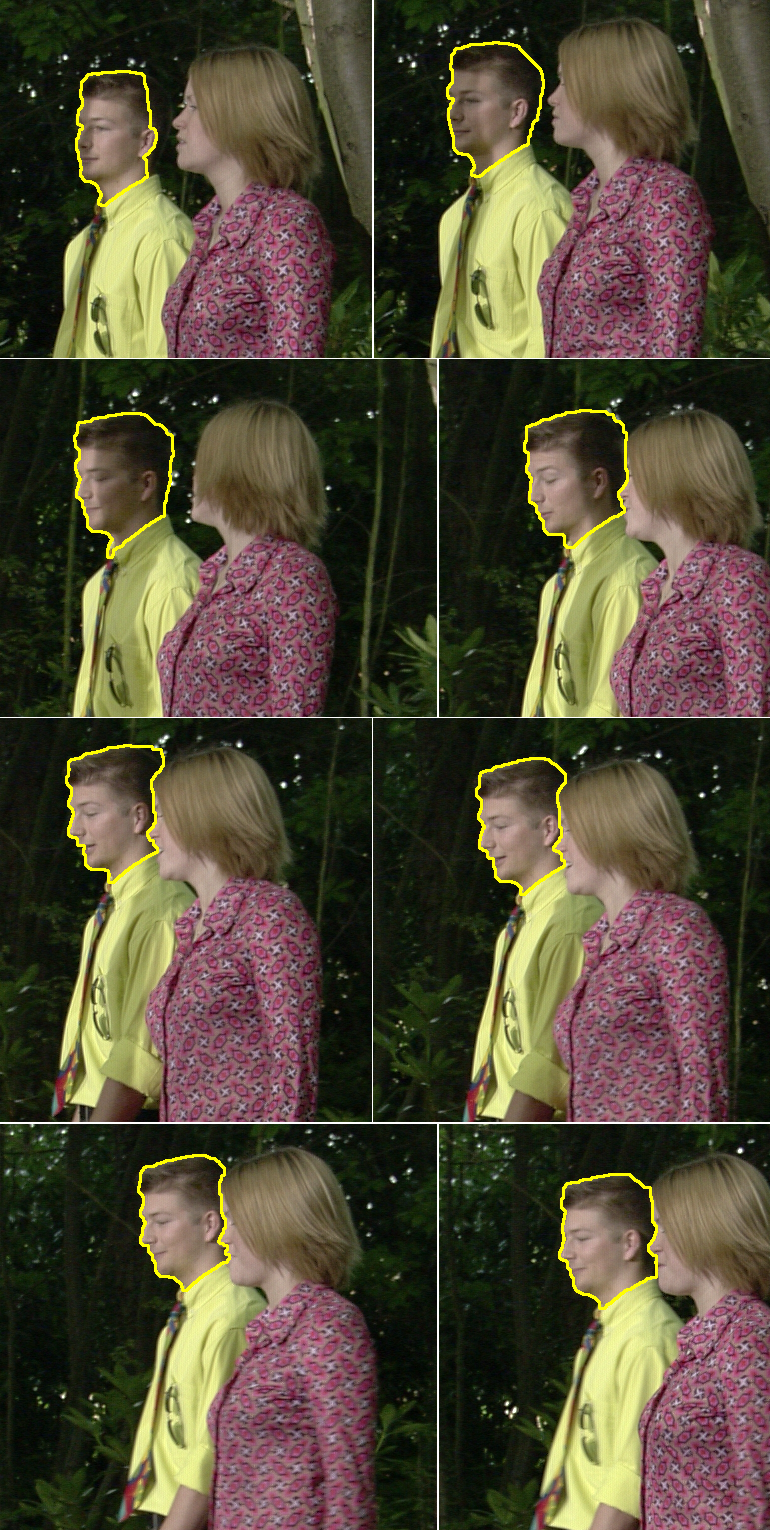
\includegraphics[height=0.66\textheight]{images/Sequence2.png}
      \caption{Segmentation through the sequence “Walking
	       Couple” (Yellow contour) initialized in the man’s head.}
      \label{figurelabel_walking}
   \end{figure}

In order to understand the effect of including super-
pixel propagation in a video sequence for object
segmentation, some results are shown in the Fig.
\ref{figurelabel_comp}. For these experiments only one iteration is
allowed in both grab-cuts initialized with only the
tracker, and the one performed with the super-pixel
propagation. Observe that in general, the contour
delineated is usually better in terms of precision and
stability for the later one.

   \begin{figure}[thpb]
      \centering
      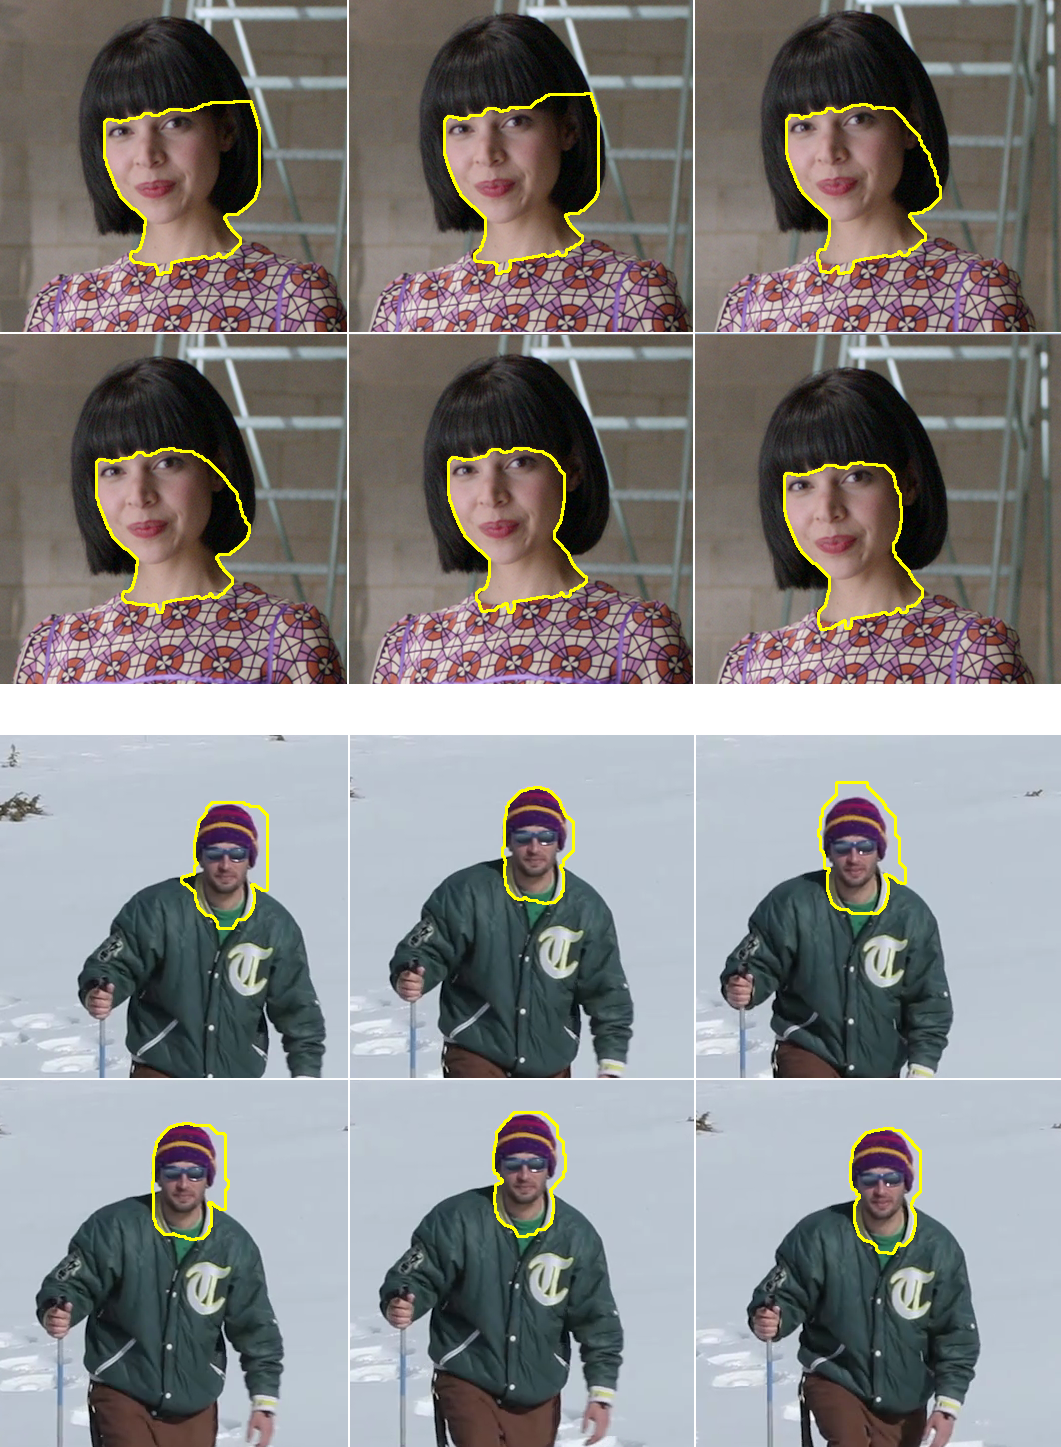
\includegraphics[height=0.4\textheight]{images/Compare.png}
      \caption{Face segmentation in the “Amelie Retro” and the
	      “Snow shoes” sequences in three different frames. For each
	       group, the Top Row: One-iteration window-based grabcut;
	       and the Bottom Row: One-iteration grabcut with super pixel
	       propagation.}
      \label{figurelabel_comp}
   \end{figure}